% Laboratorio 7 de Automatizacion - Informe IEEE editable.
\documentclass[conference,10pt]{IEEEtran}
\usepackage[T1]{fontenc}
\usepackage[utf8]{inputenc}
\usepackage[spanish,es-nodecimaldot]{babel}
\usepackage{amsmath,amssymb,mathtools}
\usepackage{booktabs,tabularx,array}
\usepackage{graphicx}
\usepackage{cite}
\usepackage{siunitx}
\usepackage{url}
\usepackage[hidelinks]{hyperref}
\usepackage{tikz}
\sisetup{output-decimal-marker={,},per-mode=symbol}

\title{Diseño e Implementación de Controladores Digitales\\
con Estimadores de Predicción y Estado Actual}
\author{\IEEEauthorblockN{Aldo Pastore}\\
\IEEEauthorblockA{Carrera de Ingeniería Electrónica\\
Universidad Católica ``Nuestra Señora de la Asunción''\\
Asignatura: Automatización --- Laboratorio N.\textsuperscript{o} 7\\
Docente: PhD. Enrique A. Vargas Cabral}}

\begin{document}
\maketitle
\begin{abstract}
Se presenta la metodología de diseño e implementación de controladores digitales
por realimentación de estados estimados para una planta analógica de segundo orden.
Se consideran un estimador de predicción y un estimador de estado actual, con dos
ubicaciones alternativas de polos del observador. El desarrollo se organiza desde
el modelo físico y la selección del tiempo de muestreo hasta la discretización,
la asignación de polos, la simulación en MATLAB y la implementación en PSoC 5LP.
La cadena de adquisición y actuación se verificó con telemetría UART y un
osciloscopio Rigol DS1202Z-E. El controlador y ambos estimadores se diseñaron
directamente con el modelo identificado en el Laboratorio 5 y
$T_s=\SI{2}{\milli\second}$. Se ensayaron las cuatro configuraciones, con 256
muestras por caso, disparo físico, cero
banderas y medición simultánea en J5/J7. Se presentan los estados estimados, el
error observable, la convergencia ante error inicial y una comparación directa
entre una referencia ideal con estados conocidos, simulación con ADC/DAC y
experimento. Los estimadores
actuales redujeron el error observable RMS respecto de sus predictores, mientras
que, al extinguirse el error de estimación, las cuatro respuestas quedaron
determinadas por los polos comunes de $A-BK$. La cuantización hizo coincidir los
niveles aplicados por predictor y actual en 46,48\,\% de las muestras E1 y
61,33\,\% de las E2, confirmando que la resolución del actuador limita la
separación experimental. El peor tiempo de cálculo representó 5,60\,\% de
$T_s$, por lo que el retardo de ejecución fue pequeño frente al período.
\end{abstract}
\begin{IEEEkeywords}
control digital, estimación de estados, observador de predicción,
observador actual, ubicación de polos, PSoC 5LP, MATLAB.
\end{IEEEkeywords}

\section{Introducción}
La realimentación completa de estados permite modificar los polos del sistema,
pero requiere conocer cada variable del vector de estado. Cuando sólo es posible
medir la salida de la planta, el diseño digital puede incluir un observador
capaz de reconstruir estados no medidos a partir del modelo, el mando y la
señal disponible \cite{samanta2024,fadali2020,astrom2020}.

La guía de esta práctica exige diseñar e implementar dos estructuras: un
estimador de predicción y un estimador de estado actual. Ambas se aplicarán a
una planta analógica de segundo orden. A diferencia del laboratorio previo,
la realimentación debe efectuarse \emph{únicamente sobre los estados estimados};
la medición física usada por el algoritmo será la salida del sistema.

La experiencia acumulada en el Laboratorio 5 proporciona una infraestructura
experimental de PSoC 5LP, MATLAB y adquisición con el Rigol DS1202Z-E. El
modelo identificado allí se adopta como base del diseño después de
contrastarlo con un ensayo abierto en esta práctica. En las cuatro
configuraciones se emplean los coeficientes obtenidos con dicho modelo, de manera que
los resultados calculados, simulados y experimentales corresponden al mismo
modelo y a las mismas ganancias.

\section{Objetivos}
\subsection{Objetivo general}
Diseñar e implementar controladores digitales para una planta analógica mediante
realimentación de estados estimados, utilizando observadores de predicción y de
estado actual, de acuerdo con la guía oficial del Laboratorio 7.

\subsection{Objetivos específicos}
\begin{enumerate}
\item Seleccionar y justificar el tiempo de muestreo antes de discretizar.
\item Obtener el modelo en espacio de estados y comprobar controlabilidad y observabilidad desde la salida medida.
\item Diseñar una ley de control común por ubicación de polos.
\item Obtener los observadores de predicción y actual; evaluar dos ubicaciones de sus polos.
\item Comparar las respuestas, errores de estimación y esfuerzos de control.
\item Implementar ambos esquemas en PSoC y confrontar los ensayos con MATLAB.
\end{enumerate}

\section{Plataforma experimental y calibración}
\subsection{Instrumentación}
La plataforma comprende un PSoC 5LP con ADC, DAC y temporizador de muestreo;
planta analógica con acondicionamiento de entrada y salida; fuente bipolar
Minipa MPL-3305M ajustada a $\pm\SI{10.2}{\volt}$; PC con MATLAB; y
osciloscopio \emph{Rigol DS1202Z-E}. Se emplearon sondas $10\times$,
acoplamiento DC, masas comunes, telemetría UART a
\SI{57600}{bit\per\second} y adquisición sincronizada. J5 midió el mando
físicamente aplicado y J7 la salida de la planta.

\subsection{Calibración y revalidación}
La Tabla~\ref{tab:calib_historica} reúne los parámetros obtenidos en el
Laboratorio 5 y reutilizados como punto de partida. Antes de cerrar el lazo se
realizó un ensayo abierto identificado de aproximadamente
\SI{50}{\milli\volt}. La variación robusta medida fue
$\Delta J5=\SI{45.38}{\milli\volt}$ y
$\Delta J7=\SI{44.45}{\milli\volt}$, equivalente a una ganancia incremental
de 0,98. La concordancia entre ambos canales confirmó polaridad, continuidad,
masa común y rango de señal antes de habilitar los controladores.

\begin{table}[t]
\centering
\caption{Parámetros de calibración adoptados del Laboratorio 5.}
\label{tab:calib_historica}
\small
\begin{tabular}{@{}ll@{}}
\toprule
Parámetro & Valor documentado \\
\midrule
Offset del ADC & \SI{2.353802067}{\volt} \\
Escala ADC/planta & \SI{0.210251951}{\volt\per\volt} \\
Ganancia de DAC (+) & 3,842612 \\
Ganancia de DAC (-) & 2,640105691 \\
Offset físico J5 & \SI{17.209}{\milli\volt} \\
Factor de escala J5/mando aplicado & 0,981710 \\
RMSE del ajuste de J7 & \SI{3.374}{\milli\volt} \\
\bottomrule
\end{tabular}
\end{table}

En cada ensayo se conservaron las ondas crudas de ambos canales, la telemetría
digital, la referencia, los estados estimados, el mando solicitado, el mando
nominal del DAC, banderas, tiempo de ejecución y metadatos de disparo. Esta
trazabilidad permite comparar resultados calculados, simulados y experimentales
sin inferir tensiones físicas únicamente a partir de códigos digitales.

\section{Modelado y discretización}
\subsection{Modelo identificado adoptado para el diseño}
El diseño utiliza el modelo identificado en el Laboratorio 5 mediante
mediciones entre J5 y J7:
\begin{equation}
G_p(s)=\frac{1.002941}{(0.00906915s+1)(0.000774399s+1)}.
\label{eq:modelo_identificado}
\end{equation}
El ensayo abierto de este laboratorio produjo una ganancia incremental cercana
a 0,98, coherente con la identificación previa. El modelo nominal se conserva
como referencia del circuito, mientras que el controlador y los estimadores se
calculan con el modelo de~\eqref{eq:modelo_identificado}.

Para mantener $x_1$ y $x_2$ en voltios y la salida $y=x_2$, se usa una
realización en cascada. La identificación entrada--salida no separa las
ganancias de ambas etapas; se conserva la ganancia nominal de la primera y se
asigna la segunda para reproducir exactamente la ganancia total
de~\eqref{eq:modelo_identificado}. Este reparto fija una base de estados y no
altera la transferencia medida.

\subsection{Selección de muestreo y modelo discreto}
Se adoptó $T_s=\SI{2}{\milli\second}$. Las cuatro capturas físicas registraron
una mediana de período de \SI{2000}{\micro\second}. La discretización ZOH del
modelo identificado resulta
\begin{equation}
A=\begin{bmatrix}0.80210&0\\-0.24963&0.075574\end{bmatrix},\qquad
B=\begin{bmatrix}-0.63161\\0.13046\end{bmatrix},
\end{equation}
\begin{equation}
C=\begin{bmatrix}0&1\end{bmatrix},\qquad D=0.
\end{equation}
Se verificaron
$\operatorname{rango}\mathcal C(A,B)=2$ y
$\operatorname{rango}\mathcal O(A,C)=2$. Por tanto, el modelo identificado
discreto es controlable y observable desde J7.

\subsection{Consistencia entre los tres niveles de validación}
El mismo modelo identificado y las mismas ganancias se usaron en: (i) el
cálculo lineal ideal; (ii) la simulación no ideal con cuantización ADC/DAC; y
(iii) el firmware programado para los ensayos. La referencia fue
\SI{50}{\milli\volt}, aplicada a partir de la muestra 32
($t=\SI{64}{\milli\second}$), con estados reiniciados durante el pretrigger.
Estas condiciones establecen una correspondencia directa entre cálculo,
simulación y banco.

\section{Diseño del controlador y estimadores}
\subsection{Realimentación de estados estimados}
Ambas arquitecturas utilizan
\begin{equation}\label{eq:control}
u[k]=-K\widehat{\mathbf{x}}[k]+N_r r[k].
\end{equation}
Con los polos de control $0.8\pm j0.25$ y el modelo identificado se obtiene
\begin{equation}
K=\begin{bmatrix}3.0726&9.3389\end{bmatrix},\qquad N_r=0.558625.
\end{equation}
La matriz $A-BK$ es común a los cuatro casos. Una vez que el error de estimación se
vuelve despreciable, ella determina la dinámica del seguimiento.

\subsection{Estimador de predicción}
La estimación disponible para el control corresponde a la predicción previa:
\begin{equation}
\widehat{\mathbf{x}}[k+1]=A\widehat{\mathbf{x}}[k]+Bu[k]
+L_p\bigl(y[k]-C\widehat{\mathbf{x}}[k]\bigr).
\end{equation}
El error evoluciona según $(A-L_pC)e[k]$. Para E1 se adoptan polos
$0.25\pm j0.05$ y para E2, $0.20\pm j0.10$. La ubicación E1 se seleccionó
entre 35 candidatas exigiendo cero abortos con el ruido medido, tolerancia a
un impulso de dos cuentas ADC y un módulo mayor que E2. El diseño produce
\begin{align}
L_{p,E1}&=\begin{bmatrix}-1.2311&0.37767\end{bmatrix}^{T},\\
L_{p,E2}&=\begin{bmatrix}-1.4923&0.47767\end{bmatrix}^{T}.
\end{align}

\subsection{Estimador de estado actual}
El estimador actual corrige la predicción con la muestra presente antes de
calcular~\eqref{eq:control}:
\begin{align}
\mathbf z[k]&=A\widehat{\mathbf{x}}[k-1]+Bu[k-1],\\
\widehat{\mathbf{x}}[k]&=\mathbf z[k]+L_a\bigl(y[k]-C\mathbf z[k]\bigr).
\end{align}
Su error corregido evoluciona con $(I-L_aC)A$. Para los mismos polos se obtiene
\begin{align}
L_{a,E1}&=\begin{bmatrix}-1.5348&-0.072302\end{bmatrix}^{T},\\
L_{a,E2}&=\begin{bmatrix}-1.8605&0.17515\end{bmatrix}^{T}.
\end{align}
Las ordenadas iniciales de predictor y actual no son directamente equivalentes:
el actual ya incorporó $y[k]$ en la muestra representada, mientras el predictor
aplicará esa innovación a la estimación siguiente.

\subsection{Límites y cuantización}
La solicitud se limita a $[-115,107]$ mV. La cadena empleada produce pasos
nominales de \SI{15.37}{\milli\volt} para la rama positiva y
\SI{10.56}{\milli\volt} para la negativa. Por tanto, diferencias pequeñas en
la acción calculada pueden desaparecer al convertirla en códigos del DAC. Esta
no linealidad se incluye en la simulación alineada con la campaña experimental.

\section{Metodología de simulación e implementación}
\subsection{Cálculo y simulación en MATLAB}
Se desarrolló un script de MATLAB que integra los tres niveles del análisis.
Primero calcula la referencia ideal con los estados
verdaderos, $u=-Kx+N_r r$, para aislar la dinámica de $A-BK$ sin observador;
luego reproduce ADC, DAC bipolar, saturaciones y cronograma del
firmware; finalmente importa las cuatro capturas UART/Rigol. Para cada caso
exporta pico y tiempo al pico, valor final, error RMS, esfuerzo máximo y RMS de
control, dispersión estacionaria del error observable, período de muestreo,
tiempo de CPU y margen temporal. También genera las trayectorias de estados, el
error observable, la convergencia ante una perturbación inicial y el análisis de
coincidencia de códigos DAC.

El error completo $\mathbf x-\widehat{\mathbf x}$ se evalúa en simulación. En
el banco solo $x_2=y$ posee una medición independiente; por ello la evidencia
experimental de error se expresa como $e_y=y-\hat x_2$, sin presentar
$x_1-\hat x_1$ como si hubiese sido medido.

\subsection{Arquitectura implementada en el PSoC}
En cada interrupción de muestreo se adquiere J7 mediante el ADC, se convierte a
unidades físicas y se actualiza el estimador seleccionado. Luego se calcula la
ley~\eqref{eq:control}, se limita la solicitud a la región validada y se escribe
el DAC. La UART registra referencia, salida, estados estimados, innovación,
mando solicitado, mando nominal, banderas, intervalo y tiempo de ejecución.

Los coeficientes identificados se integraron con límites conservadores de
$[-115,107]$ mV, detección abortiva de saturación y comprobación posterior a la
cuantización. Las cuatro combinaciones de arquitectura y ubicación compilaron
en PSoC Creator 4.4 y se programaron sucesivamente. Ninguna
ejecución generó banderas. Al finalizar se volvió a compilar y programar
MONITOR, con el DAC en cero y todas las autorizaciones de lazo cerrado
deshabilitadas; después se apagó la fuente bipolar.

\subsection{Protocolo de medición}
Antes del lazo cerrado se verificaron masas, sondas $10\times$, polaridad,
salida nula, respuesta abierta, período de muestreo y retorno seguro. Para cada
configuración se programó el firmware correspondiente, se rearmó el sistema y
se adquirieron simultáneamente 256 registros UART y 1200 puntos por canal del
Rigol. Los metadatos de cada adquisición permitieron verificar el modo, la
familia de polos, el modelo identificado, el disparo físico, la ausencia de
disparo forzado, $T_s$ y las banderas. Las ondas crudas se conservaron sin
modificaciones; el suavizado mostrado en una figura se utiliza únicamente para
visualización.

\section{Resultados y discusión}
\subsection{Comparación calculada, simulada y experimental}
La Tabla~\ref{tab:comparacion_integrada} aplica una misma metodología a las
cuatro configuraciones identificadas. C denota cálculo lineal, S la simulación
con ADC/DAC y E el experimento. En C se realimentan directamente los estados
verdaderos, por lo que esta columna es la referencia ideal de $A-BK$, no la
salida de otro estimador. El pico se busca en los primeros
\SI{100}{\milli\second} del transitorio; el valor final es la media de las
últimas 50 muestras. La matriz aumentada posee $\rho=0.8382$ en los cuatro
casos porque los polos de control son comunes y los polos del observador
permanecen desacoplados por el principio de separación.

\begin{table*}[t]
\centering
\caption{Comparación directa con el modelo identificado. Amplitudes, RMSE y
mando en mV; $t_p$ experimental en ms.}
\label{tab:comparacion_integrada}
\small
\resizebox{\textwidth}{!}{%
\begin{tabular}{@{}lrrrrrrrrrr@{}}
\toprule
Caso & Pico C & Pico S & Pico E & Final C & Final S & Final E & RMSE S--E & RMS $e_y$ E & $|u_{apl}|_{\max}$ E & $t_p$ E\\
\midrule
Predictor E1 & 58.01 & 62.55 & 65 & 50.00 & 61.66 & 46.12 & 13.35 & 2.91 & 77 & 40\\
Actual E1    & 58.01 & 61.66 & 65 & 50.00 & 61.66 & 49.62 & 12.15 & 2.29 & 92 & 18\\
Predictor E2 & 58.01 & 62.55 & 65 & 50.00 & 61.66 & 46.24 & 13.46 & 2.91 & 77 & 20\\
Actual E2    & 58.01 & 64.17 & 60 & 50.00 & 46.25 & 50.30 &  6.20 & 1.77 & 92 & 14\\
\bottomrule
\end{tabular}}
\end{table*}

La referencia ideal coincide en los cuatro casos: al desaparecer el error de
estimación, la dinámica restante es la de $A-BK$. La simulación no ideal
reproduce el crecimiento inicial, pero presenta niveles estacionarios
cuantizados. El experimento conserva la forma del transitorio y queda a uno o
pocos niveles del DAC/ADC alrededor de la referencia. En las condiciones
ensayadas, Actual E2 obtuvo la menor RMSE simulación--experimento y el menor
error observable RMS. La diferencia de régimen se asocia al efecto conjunto de
cuantización, ruido y calibración, no a una modificación de los polos de control.

\begin{figure*}[t]
\centering
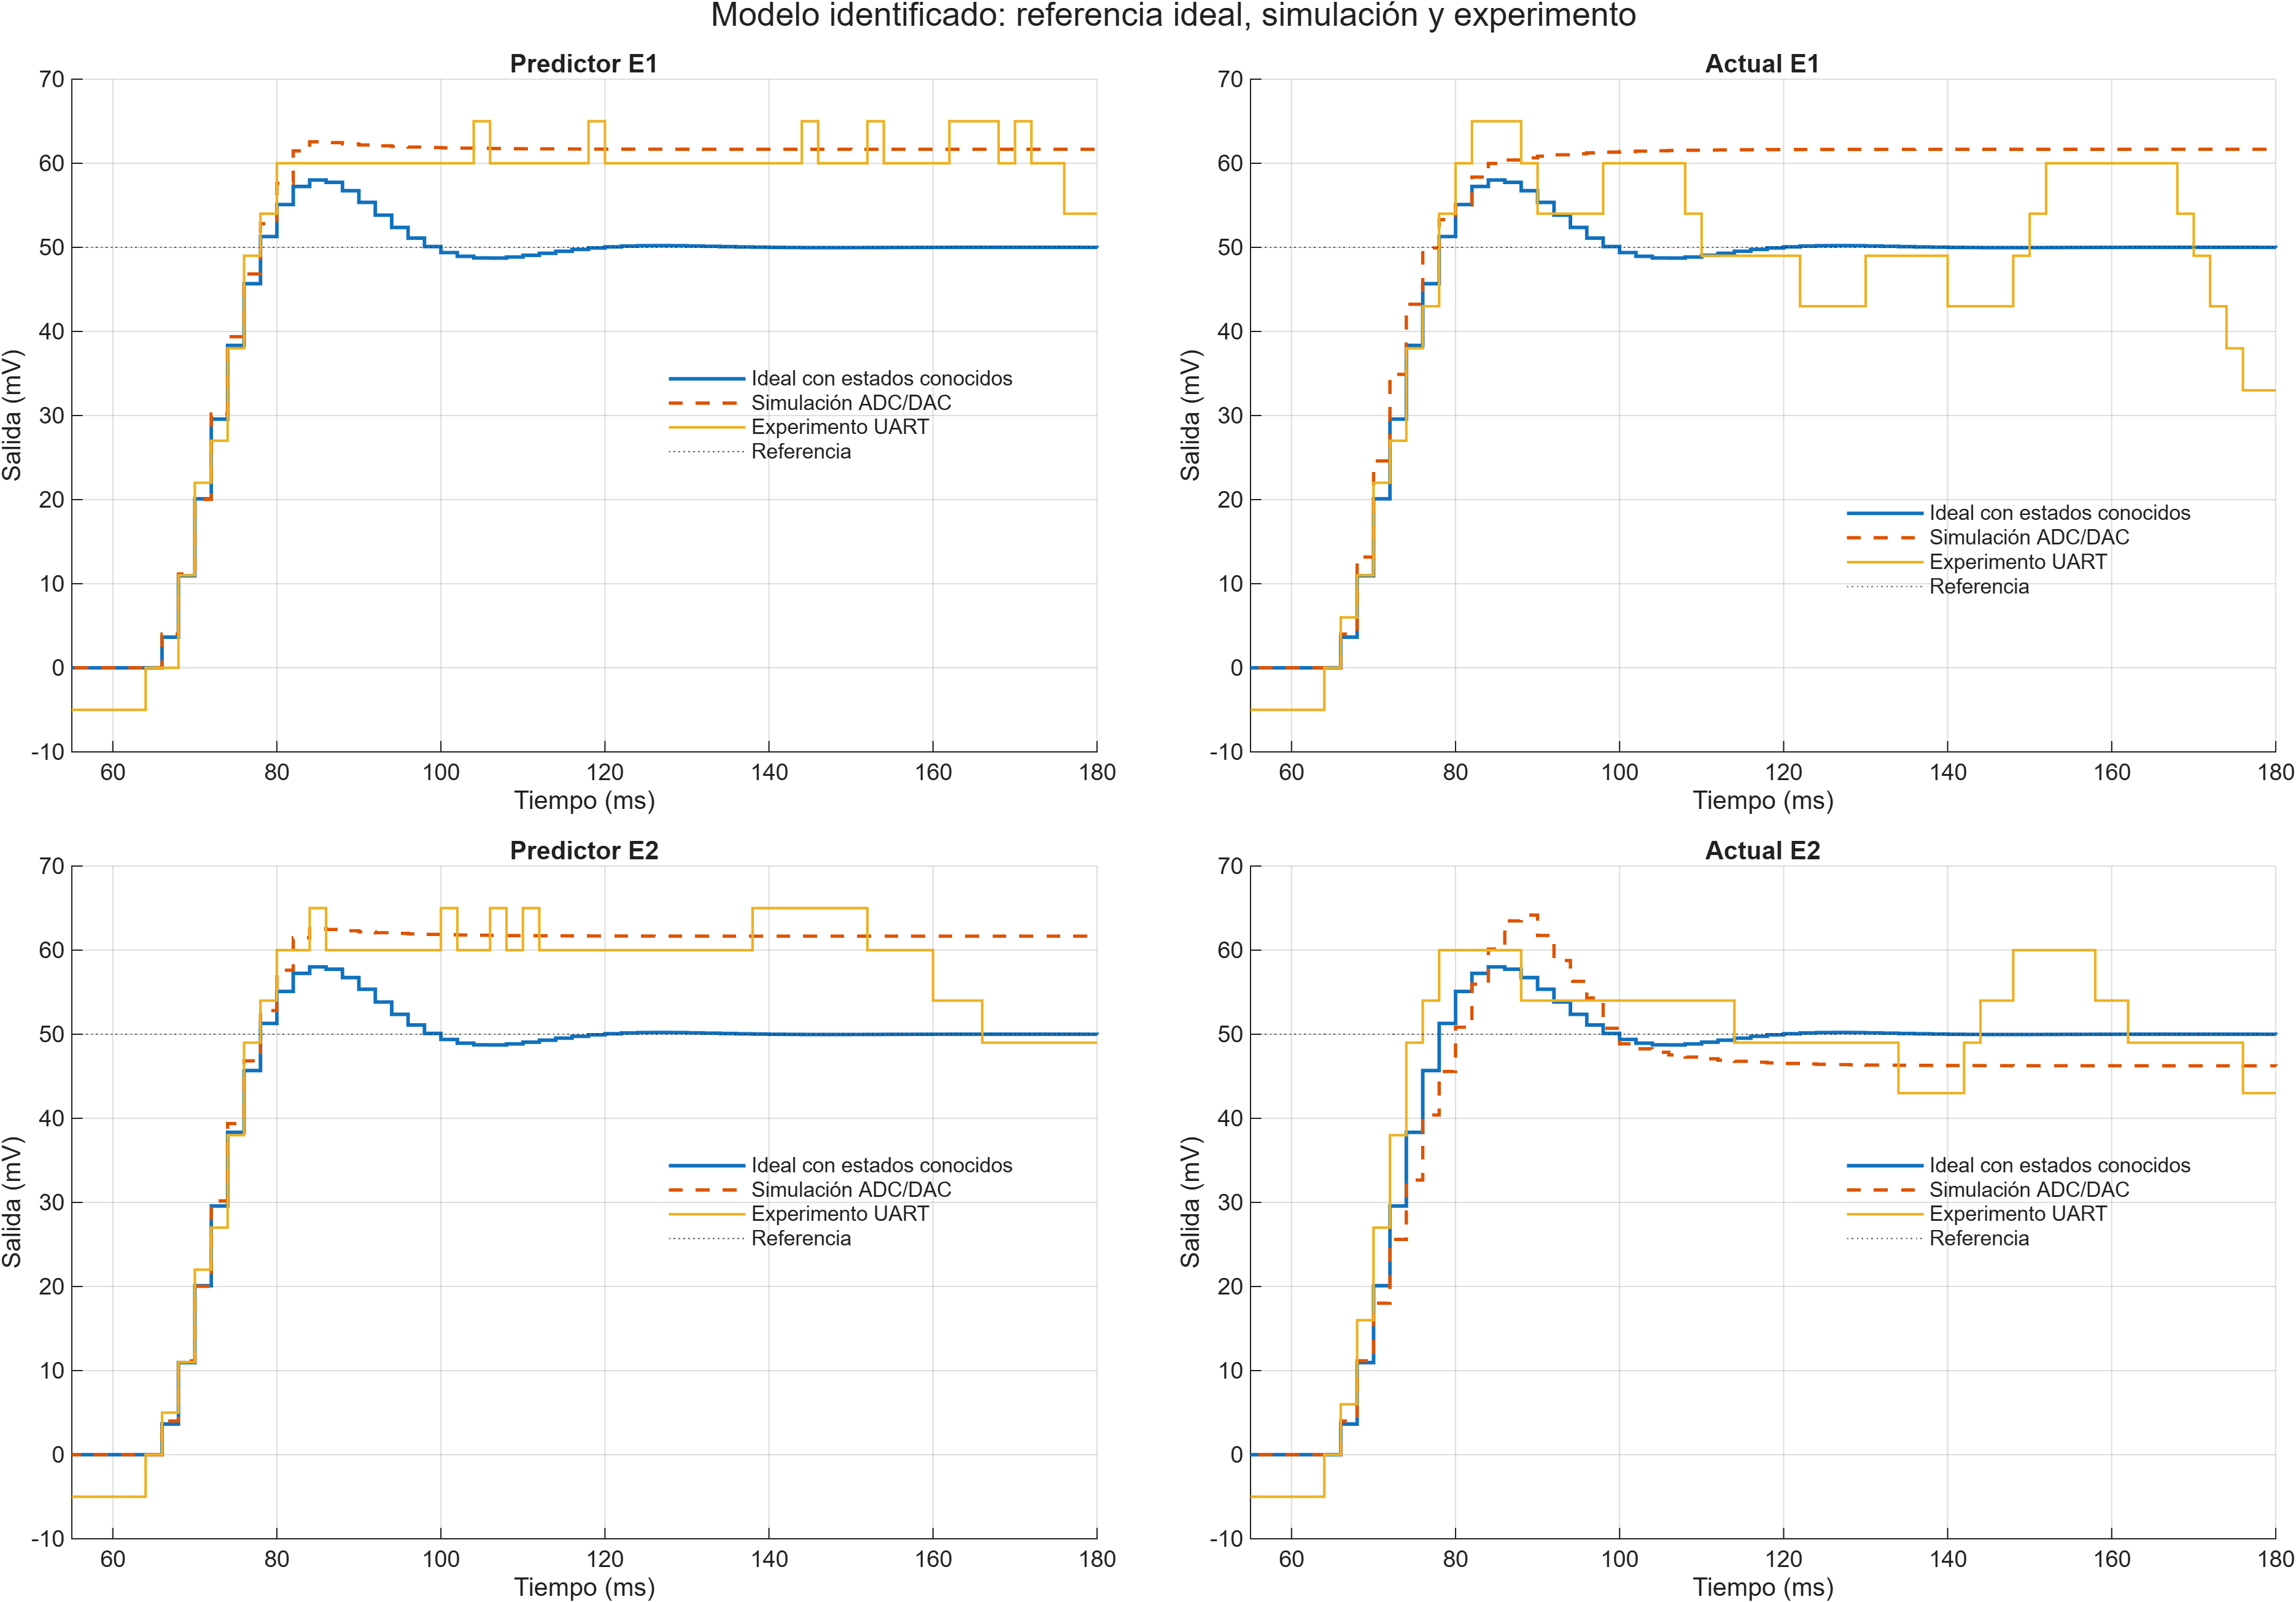
\includegraphics[width=\textwidth]{../05_Resultados/Validacion_Integrada_20261124/figuras/comparacion_calculada_simulada_experimental_4_casos.png}
\caption{Comparación de la referencia ideal con estados conocidos, la simulación
no ideal y la telemetría experimental para las cuatro configuraciones.}
\label{fig:comparacion_sim_exp}
\end{figure*}

La Tabla~\ref{tab:esfuerzo_ruido_tiempo} complementa los máximos con el valor
RMS del mando aplicado desde el escalón. La desviación estándar de $e_y$ usa
las últimas 50 muestras y separa la dispersión del sesgo. La fracción temporal
se define como $100t_{\mathrm{CPU,max}}/T_s$ y el margen como su complemento.

\begin{table}[t]
\centering
\caption{Esfuerzo, dispersión observable y margen temporal experimentales.}
\label{tab:esfuerzo_ruido_tiempo}
\small
\resizebox{\columnwidth}{!}{%
\begin{tabular}{@{}lrrrr@{}}
\toprule
Caso & $u_{\mathrm{RMS}}$ (mV) & $\sigma_{e_y}$ (mV) & CPU/$T_s$ (\%) & Margen (\%)\\
\midrule
Predictor E1 & 50,35 & 3,38 & 5,60 & 94,40\\
Actual E1    & 53,28 & 2,49 & 5,50 & 94,50\\
Predictor E2 & 49,78 & 3,49 & 5,55 & 94,45\\
Actual E2    & 51,03 & 1,72 & 5,55 & 94,45\\
\bottomrule
\end{tabular}}
\end{table}

Actual E2 presentó la menor dispersión de $e_y$ en esta campaña. Este resultado
se limita a una ejecución por caso y no se generaliza como una propiedad
universal frente al ruido. Los cuatro valores de $u_{\mathrm{RMS}}$ fueron
similares y el cálculo ocupó como máximo el 5,60\,\% de $T_s$.

\subsection{Estados estimados y errores en las cuatro configuraciones}
La Fig.~\ref{fig:estados_estimados} presenta $\hat x_1$, $\hat x_2$ y la salida
medida. $\hat x_1$ es un estado interno de la realización identificada; sus
valores negativos no representan una tensión medida directamente. La
Fig.~\ref{fig:errores_estimacion} muestra el error observable
$e_y=y-\hat x_2$. Desde el escalón, los RMS fueron 2,91; 2,29; 2,91 y
\SI{1.77}{\milli\volt} para Predictor E1, Actual E1, Predictor E2 y Actual E2.
En ambas familias el estimador actual redujo el RMS respecto del predictor,
coherente con el uso de la muestra presente antes de calcular el mando.

\begin{figure*}[t]
\centering
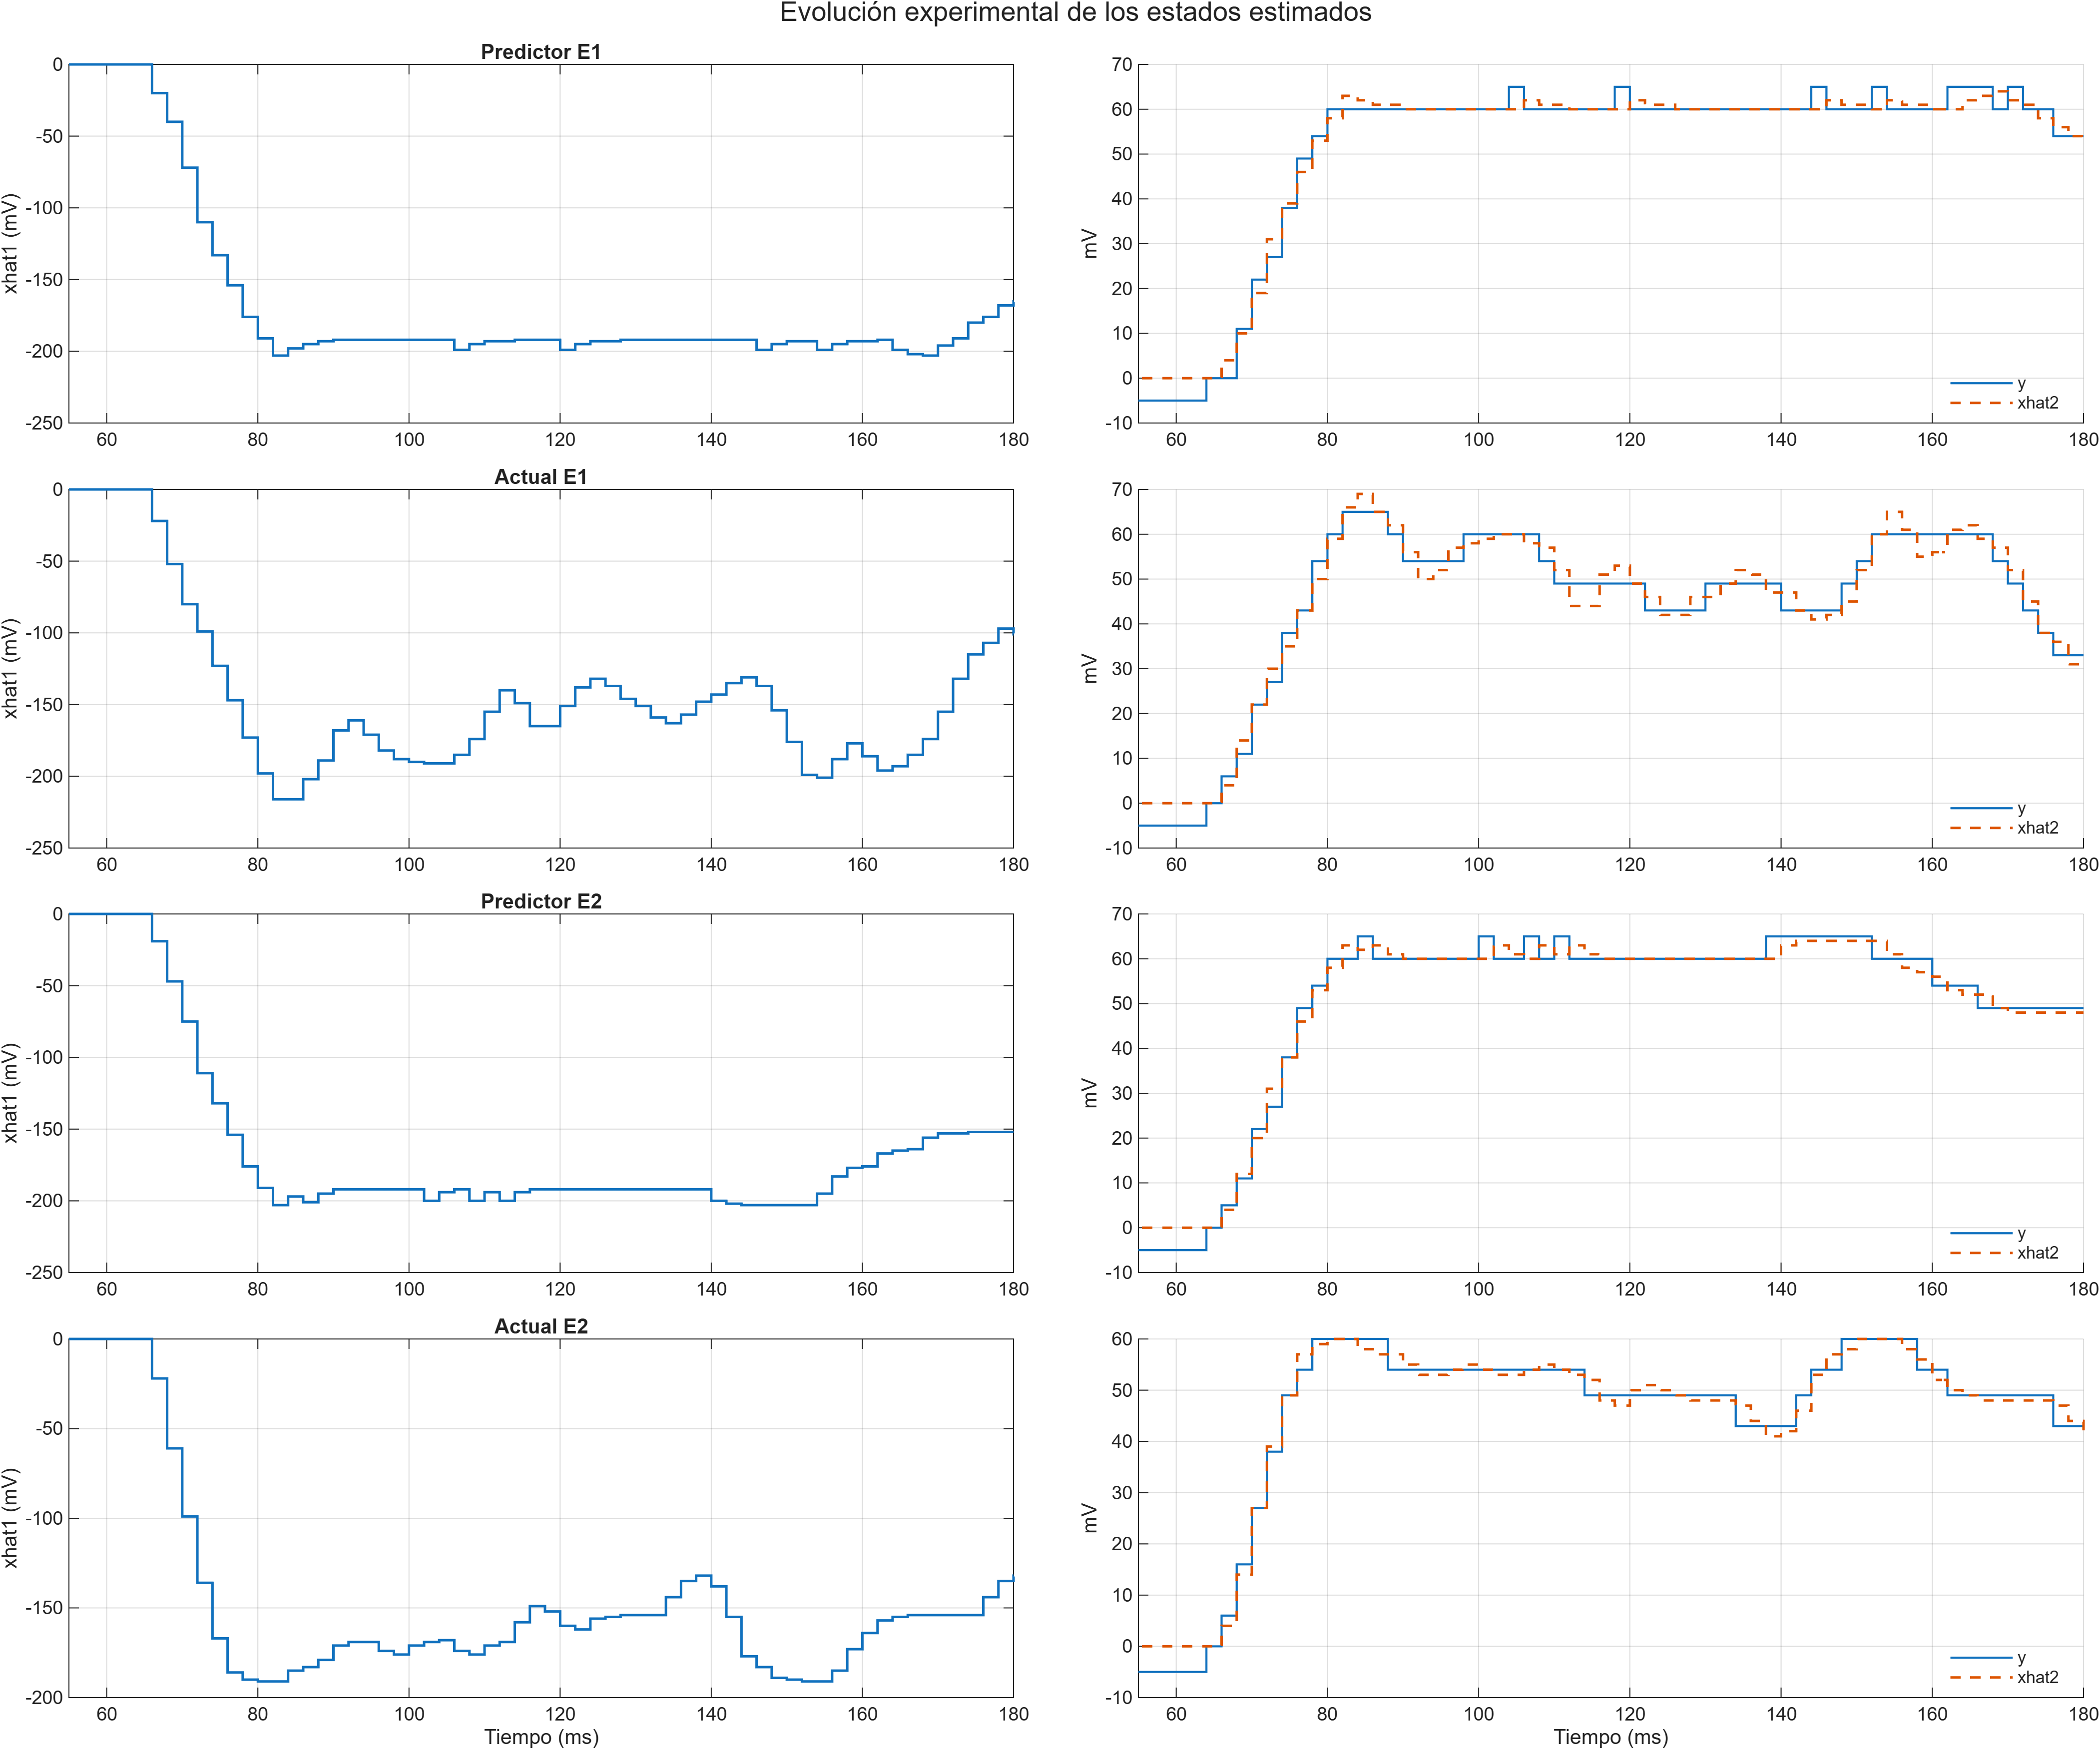
\includegraphics[width=\textwidth]{../05_Resultados/Validacion_Integrada_20261124/figuras/estados_estimados_experimentales_4_casos.png}
\caption{Evolución experimental de los estados estimados. La salida medida se
superpone con $\hat x_2$; $\hat x_1$ no posee medición independiente.}
\label{fig:estados_estimados}
\end{figure*}

\begin{figure*}[t]
\centering
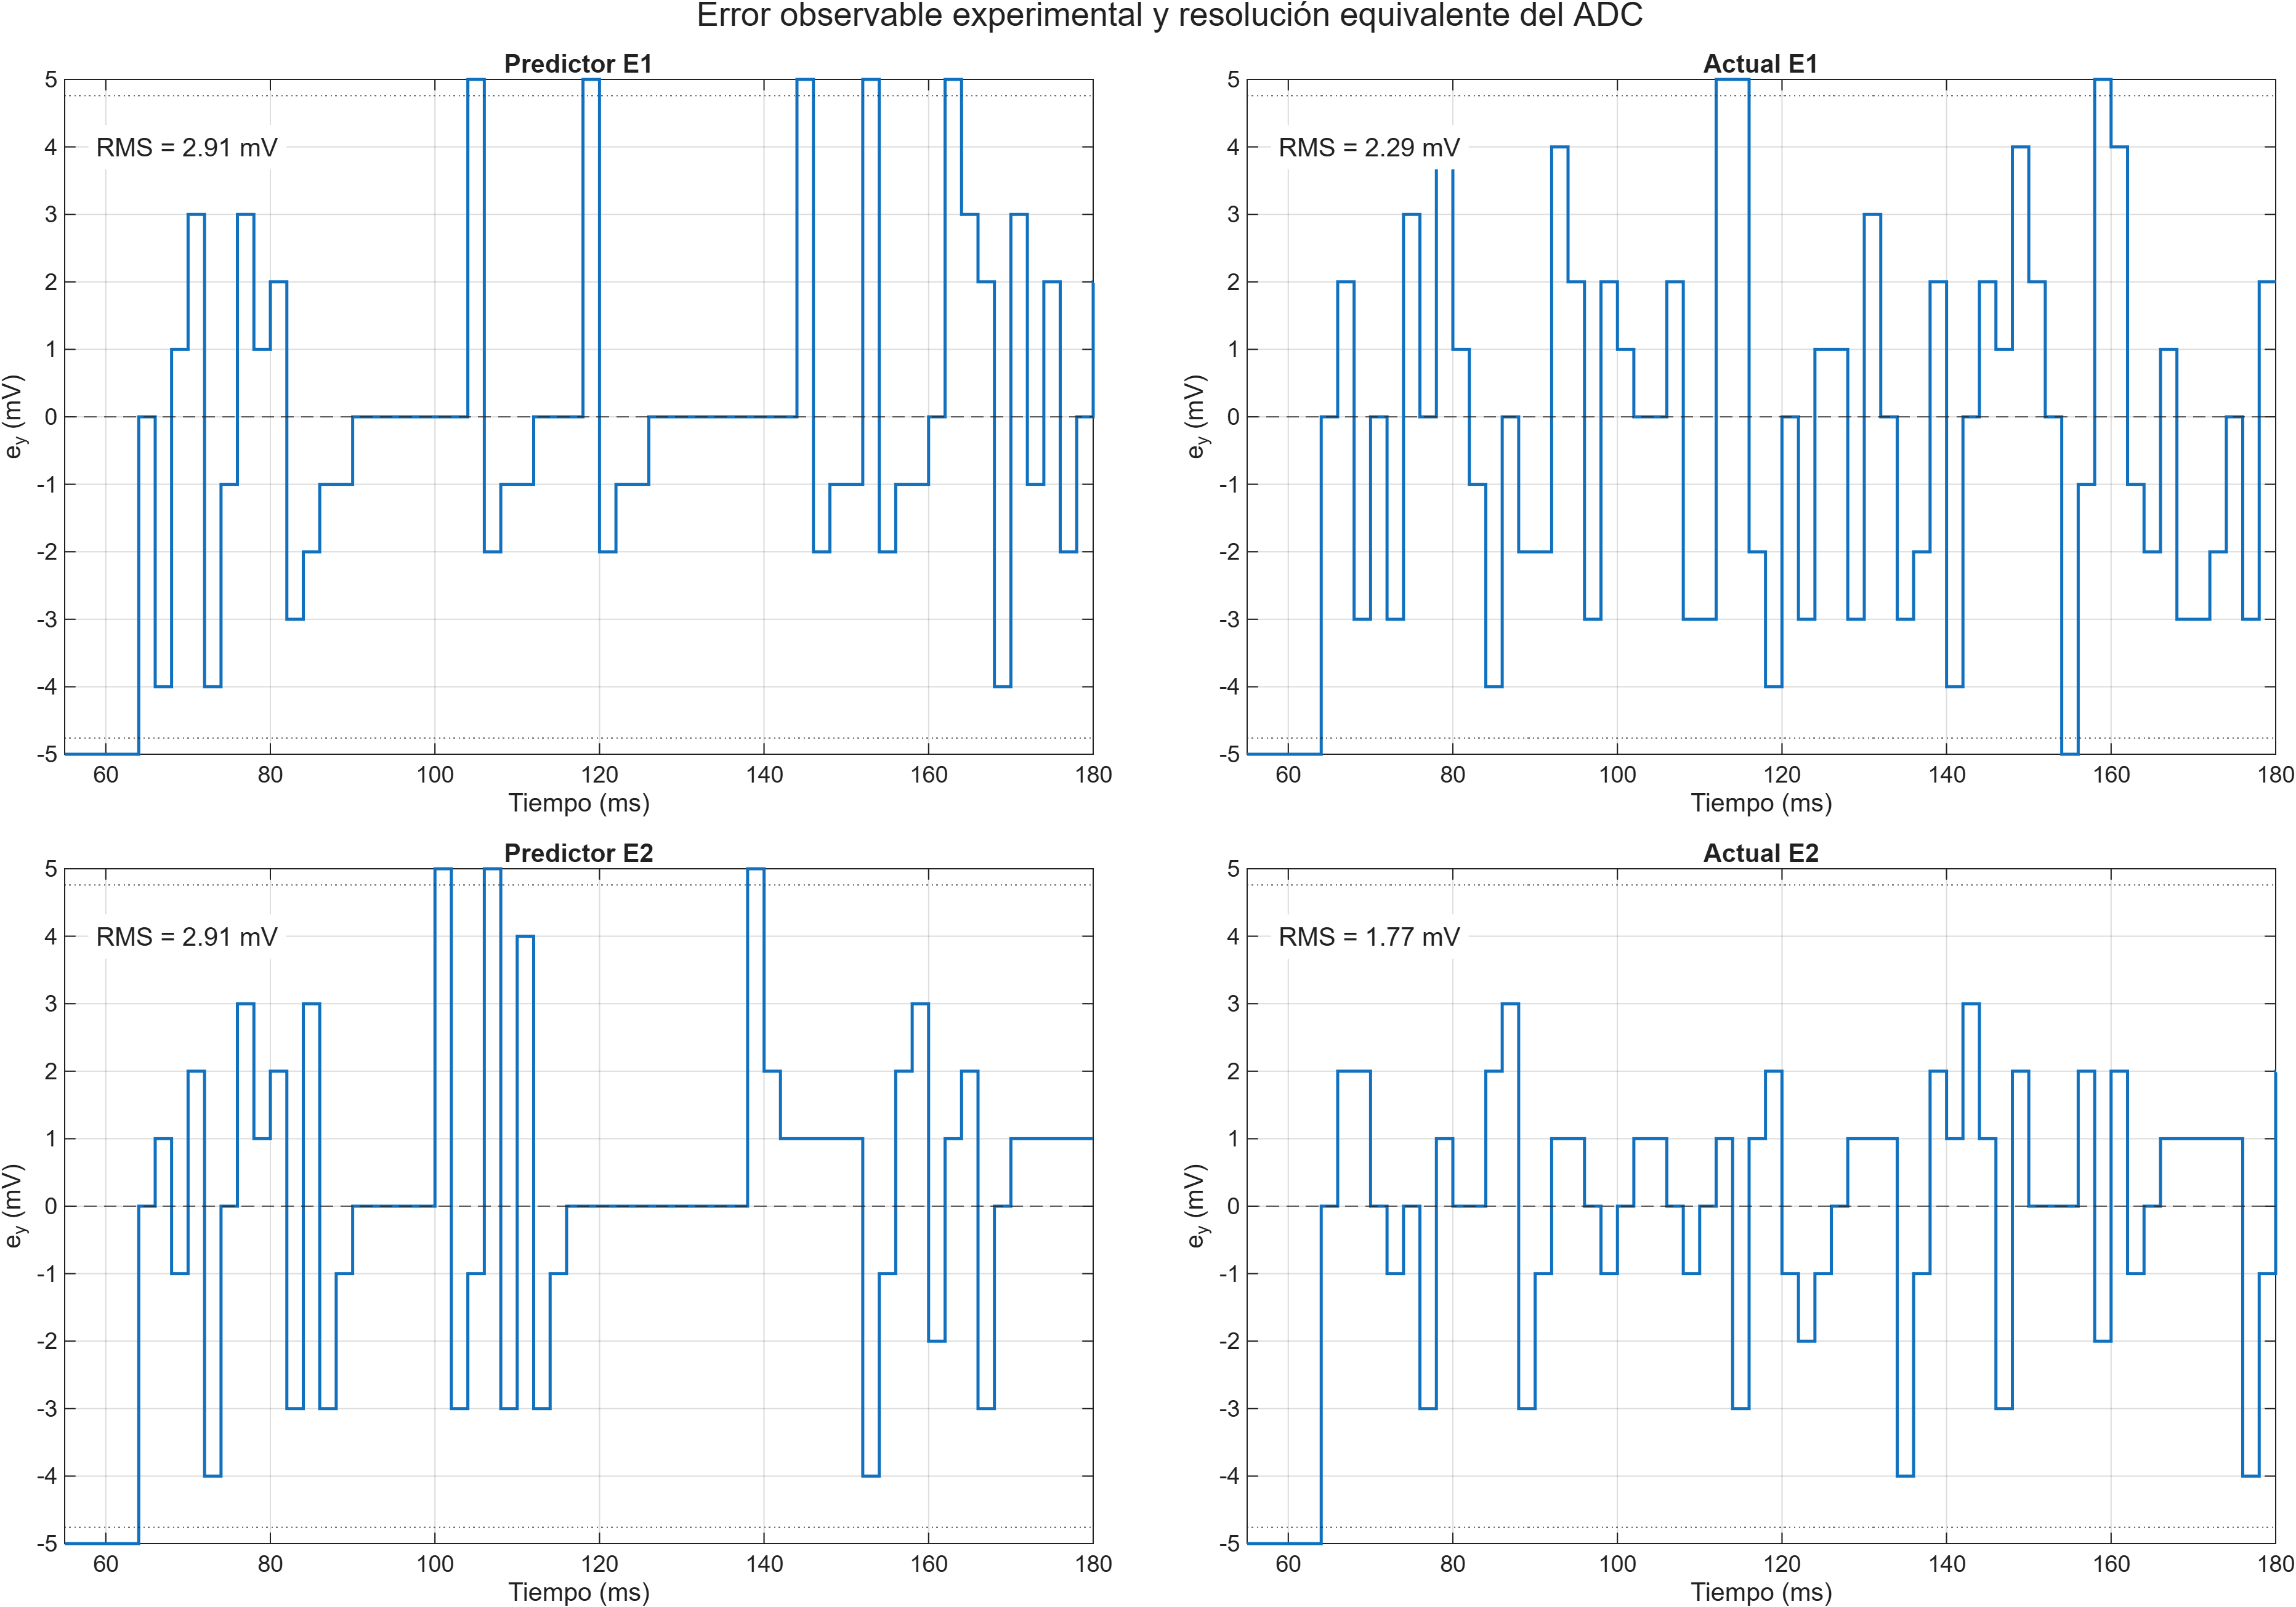
\includegraphics[width=\textwidth]{../05_Resultados/Validacion_Integrada_20261124/figuras/errores_estimacion_experimentales_4_casos.png}
\caption{Error observable experimental. Las líneas punteadas indican la
resolución equivalente aproximada de una cuenta ADC (\SI{4.76}{\milli\volt}).}
\label{fig:errores_estimacion}
\end{figure*}

\subsection{Rapidez de convergencia y efecto de la muestra presente}
Se emplearon dos indicadores distintos. Para los polos del observador se calculó
\begin{equation}
N_{2\%}=\left\lceil\frac{\log(0.02)}{\log\rho_o}\right\rceil,
\qquad t_{2\%}=N_{2\%}T_s,
\end{equation}
donde $\rho_o$ es el mayor módulo de los polos asignados. En la simulación de
la perturbación se definió $t_c$ como el primer instante a partir del cual
$\|e[k]\|_2<10^{-4}$ V se cumple para todas las muestras restantes. Por tanto,
$t_{2\%}$ y $t_c$ son referencias complementarias y no métricas idénticas.

\begin{table}[t]
\centering
\caption{Convergencia teórica y simulada del error de estimación.}
\label{tab:convergencia_teorica}
\small
\resizebox{\columnwidth}{!}{%
\begin{tabular}{@{}lrrrrr@{}}
\toprule
Familia & $\rho_o$ & $N_{2\%}$ & $t_{2\%}$ (ms) & $t_c$ Pred. (ms) & $t_c$ Actual (ms)\\
\midrule
E1, $0.25\pm j0.05$ & 0,25495 & 3 & 6 & 6 & 6\\
E2, $0.20\pm j0.10$ & 0,22361 & 3 & 6 & 8 & 8\\
\bottomrule
\end{tabular}}
\end{table}

Para aislar el transitorio de estimación se simuló
$\hat x[0]-x[0]=[0.02\;-0.01]^T$ V. Predictor y actual alcanzaron
persistentemente $\|e\|_2<10^{-4}$ en 6 ms para E1 y en 8 ms para E2. La
ventaja del estimador actual aparece inmediatamente después de incorporar
$y[k]$: el error inicial corregido fue 11,69 mV frente a 22,36 mV en E1, y
8,37 mV frente a 22,36 mV en E2. Aunque el cálculo modal redondea ambas familias
a tres muestras, el cruce de un umbral absoluto depende también de la dirección
del error inicial y de la combinación modal; la tasa asintótica queda determinada
por los polos asignados.
Una vez extinguido ese error, las cuatro curvas de salida obedecen a $A-BK$.

\begin{figure*}[t]
\centering
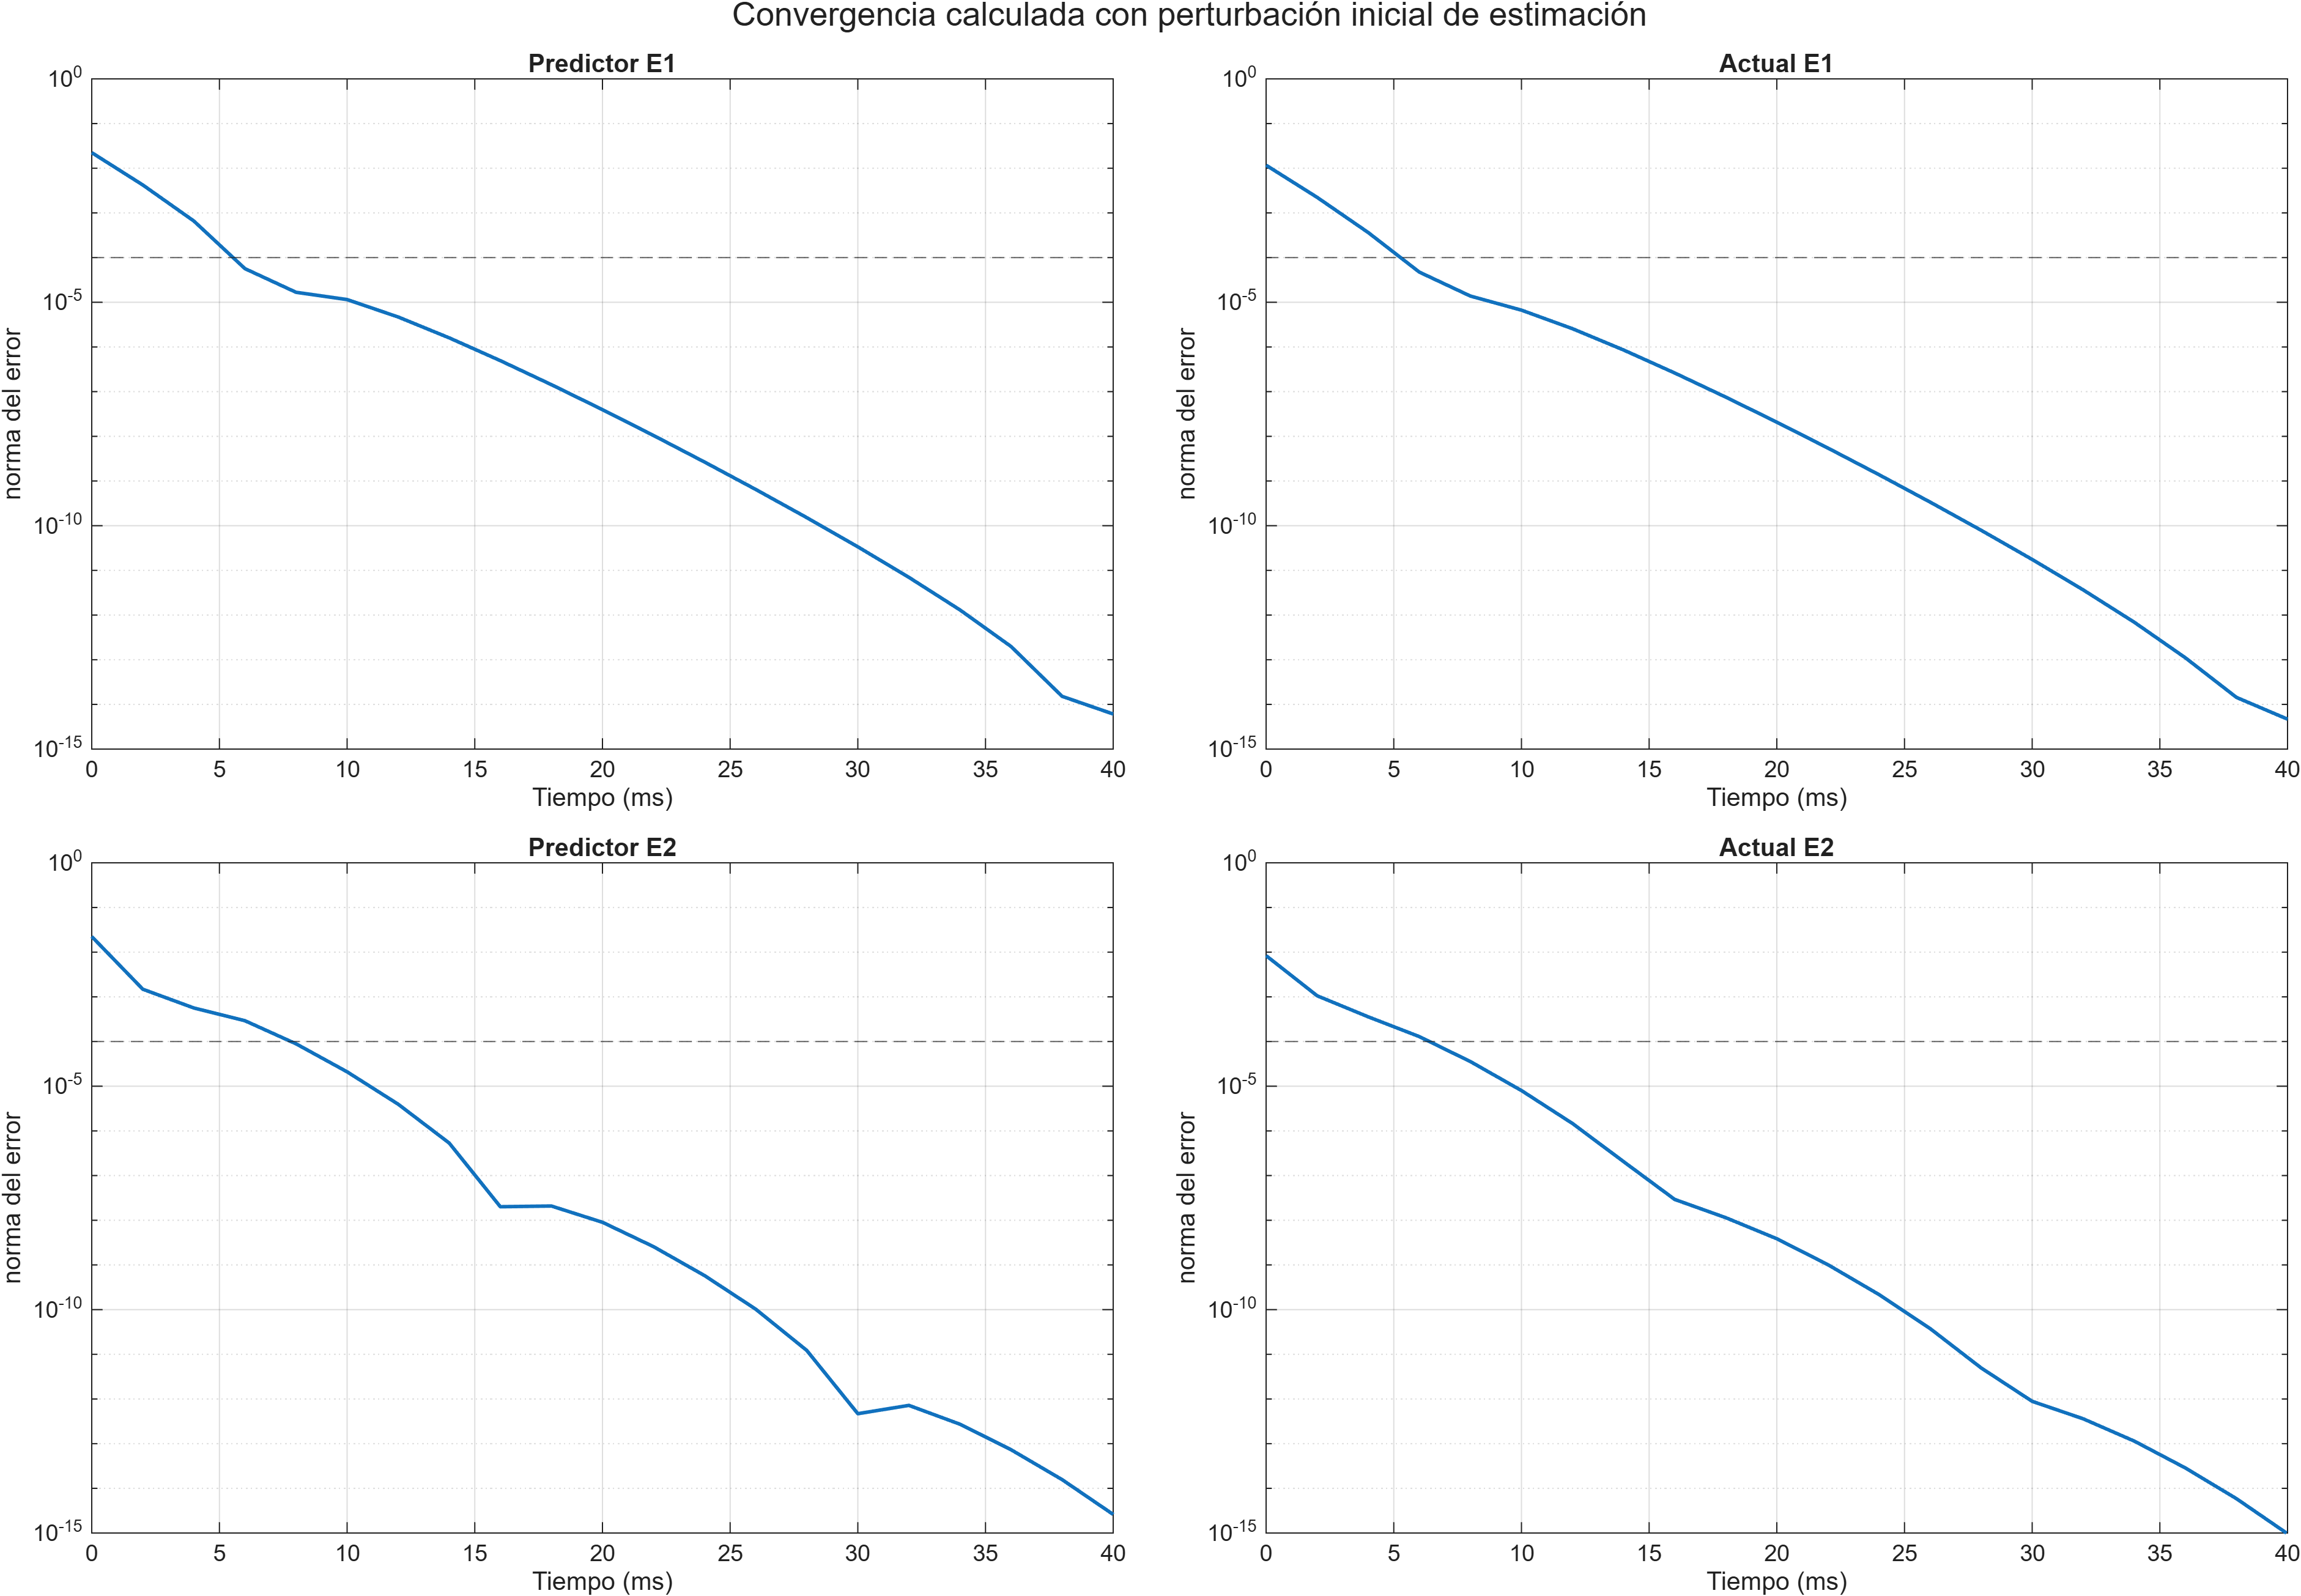
\includegraphics[width=\textwidth]{../05_Resultados/Validacion_Integrada_20261124/figuras/convergencia_rediseno_identificado_4_casos.png}
\caption{Convergencia calculada del error de estado ante la misma perturbación
inicial, con escala vertical común.}
\label{fig:convergencia_identificada}
\end{figure*}

\subsection{Validación física simultánea}
El Rigol confirmó que J5 y J7 cambiaron simultáneamente al terminar cada
ensayo. La Tabla~\ref{tab:rigol} usa las medianas del primer y último 20\,\% de
cada registro para evitar que el ruido de alta frecuencia sesgue la amplitud.
Las razones $\Delta J7/\Delta J5$ permanecieron entre 0,974 y 1,064.

\begin{table}[t]
\centering
\caption{Variaciones físicas medidas por el Rigol.}
\label{tab:rigol}
\small
\begin{tabular}{@{}lrrr@{}}
\toprule
Caso & $\Delta J5$ (mV) & $\Delta J7$ (mV) & Razón\\
\midrule
Predictor E1 & 44 & 46,0 & 1,046\\
Actual E1    & 50 & 53,2 & 1,064\\
Predictor E2 & 46 & 44,8 & 0,974\\
Actual E2    & 48 & 50,0 & 1,042\\
\bottomrule
\end{tabular}
\end{table}

\begin{figure*}[t]
\centering
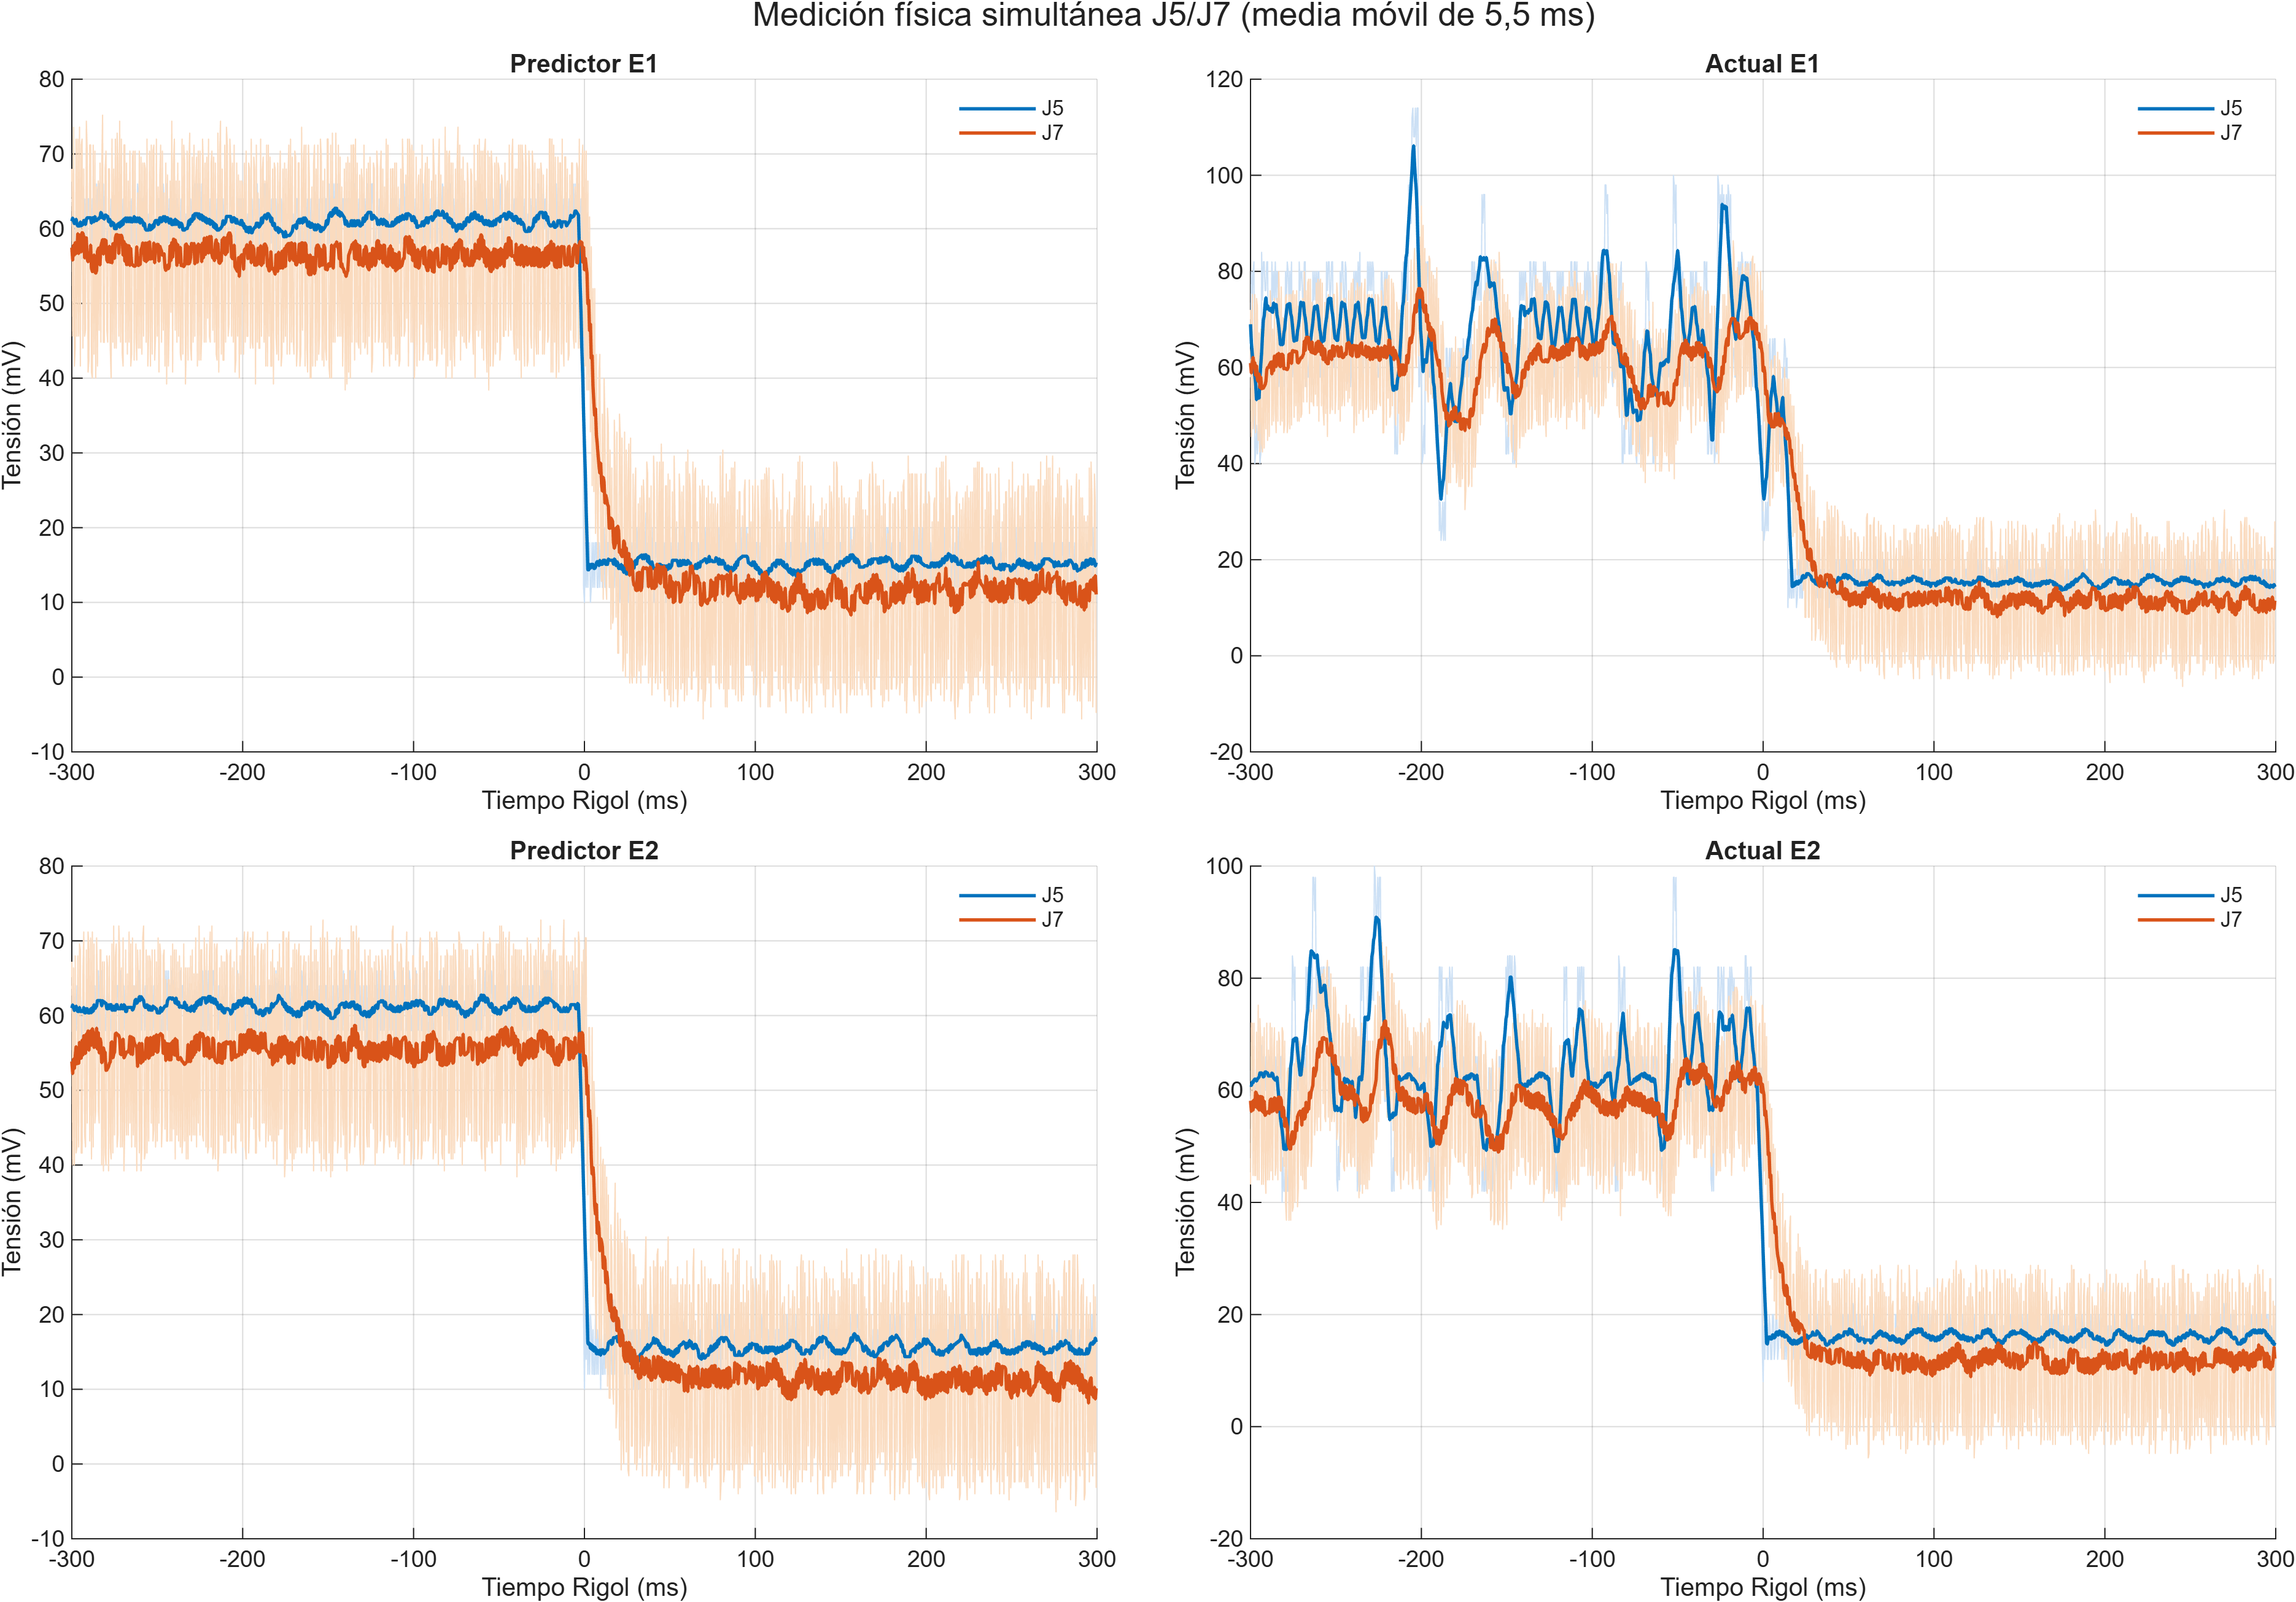
\includegraphics[width=\textwidth]{../05_Resultados/Validacion_Integrada_20261124/figuras/mediciones_fisicas_Rigol_4_casos.png}
\caption{Ondas J5/J7 al retorno seguro. Las líneas intensas muestran una media
móvil de 5,5 ms; los datos crudos se preservan en segundo plano.}
\label{fig:rigol_fisico}
\end{figure*}

\subsection{Resolución del actuador}
La Tabla~\ref{tab:cuantizacion} compara predictor y actual por índice de muestra
dentro de cada familia. ``Compresión'' es la fracción de solicitudes diferentes
que terminó en el mismo nivel del DAC. Aun cuando los mandos calculados difieren,
una proporción importante se convierte en el mismo valor físico.

\begin{table}[t]
\centering
\caption{Coincidencia de acciones por cuantización del DAC.}
\label{tab:cuantizacion}
\small
\begin{tabular}{@{}lrrr@{}}
\toprule
Par & Mismo DAC & Solicitud distinta, mismo DAC & Compresión\\
\midrule
E1 & 46,48\,\% & 32,42\,\% & 37,73\,\%\\
E2 & 61,33\,\% & 45,70\,\% & 54,17\,\%\\
\bottomrule
\end{tabular}
\end{table}

Los pasos nominales fueron \SI{15.37}{\milli\volt} en la rama positiva y
\SI{10.56}{\milli\volt} en la negativa. Las diferencias solicitadas medias
entre arquitecturas fueron 9,44 mV para E1 y 6,34 mV para E2, magnitudes del
orden de un paso. Con una referencia de solo \SI{50}{\milli\volt}, esta
resolución reduce la capacidad de distinguir estructuras a partir de la salida.

\subsection{Verificación temporal y alcance experimental}
Cada captura contiene 256 muestras, mediana de
\SI{2000}{\micro\second}, tiempo máximo de CPU entre 110 y
\SI{112}{\micro\second}, cero banderas y disparo físico sin forzado. Los
metadatos registran el modelo, la arquitectura y la ubicación de polos de cada
ensayo. El peor caso ocupó 5,60\,\% del período y dejó 94,40\,\% de
margen, por lo que el retardo de cómputo no fue comparable con $T_s$. Por tanto,
la actualización del DAC se completó con holgura dentro de cada período.

La comparación experimental corresponde a una ejecución por configuración con
una referencia de \SI{50}{\milli\volt}. Como $x_1$ no dispone de una medición
independiente, su error se analiza en simulación; en el banco se utiliza
$e_y=y-\hat x_2$. La UART registra el transitorio completo y el osciloscopio
corrobora la amplitud física y la simultaneidad de J5 y J7. Los CSV crudos, las
métricas y el script se conservan para reproducir el análisis.

\clearpage
\raggedbottom
\section{Conclusiones}
El modelo identificado a partir de las mediciones entre J5 y J7 proporcionó la
base común para calcular el controlador, los observadores y las simulaciones.
Los mismos coeficientes se programaron en el PSoC para las cuatro
configuraciones. Los registros de 256 muestras mantuvieron un período de
\SI{2}{\milli\second}, no presentaron banderas y contaron con disparo físico y
medición simultánea de J5 y J7.

La comparación directa utilizó una referencia ideal con estados verdaderos y
mostró la dinámica de $A-BK$ sin intervención de un observador. Una vez que el
error de estimación se hace despreciable, las respuestas comparten dicha
dinámica; las diferencias sostenidas entre simulación y banco se explican por
la cuantización, el ruido y la calibración. Los valores finales experimentales
fueron 46,12; 49,62; 46,24 y \SI{50.30}{\milli\volt}, con picos entre 60 y
65 mV.

La evolución de los estados estimados mostró que $\hat x_2$ acompaña la salida
medida, mientras que $\hat x_1$ representa el estado interno no medido. El error
observable RMS descendió de 2,91 a \SI{2.29}{\milli\volt} entre Predictor y
Actual E1, y de 2,91 a \SI{1.77}{\milli\volt} en E2. Ante la misma perturbación
inicial, el uso de la muestra presente redujo inmediatamente la norma del error:
11,69 frente a 22,36 mV en E1 y 8,37 frente a 22,36 mV en E2. Después de la
convergencia no corresponde esperar dinámicas distintas, pues domina $A-BK$.

La estimación modal al 2\,\% produjo tres muestras, o 6 ms, para E1 y E2. Con
el criterio persistente $\|e\|_2<10^{-4}$ V, la perturbación considerada
convergió en 6 ms para E1 y 8 ms para E2. Esta diferencia muestra que el cruce
de un umbral finito también depende de la dirección del error inicial y de la
combinación modal.

Los mandos aplicados tuvieron valores RMS entre 49,78 y 53,28 mV. En las
últimas 50 muestras, la desviación estándar del error observable fue 3,38;
2,49; 3,49 y 1,72 mV para Predictor E1, Actual E1, Predictor E2 y Actual E2.
Estos valores describen las condiciones de los ensayos realizados y muestran
una menor dispersión para Actual E2. El peor tiempo de CPU fue 112 $\mu$s,
equivalente al 5,60\,\% de $T_s$, con un margen temporal mínimo de 94,40\,\%.

La resolución del actuador explica parte de la semejanza entre las respuestas
experimentales. El nivel aplicado coincidió entre predictor y actual en
46,48\,\% de las muestras E1 y 61,33\,\% de las E2; entre solicitudes distintas,
la compresión al mismo código alcanzó 37,73\,\% y 54,17\,\%. Los pasos de
10,56--15,37 mV son grandes frente a la referencia de
\SI{50}{\milli\volt}, de modo que diferencias de mando pueden resultar
invisibles en la salida física.


\begin{thebibliography}{9}
\bibitem{samanta2024} B. Samanta, \emph{Introduction to Digital Control: An Integrated Approach}. Springer, 2024.
\bibitem{fadali2020} M. S. Fadali y A. Visioli, \emph{Digital Control Engineering: Analysis and Design}, 3.\textsuperscript{a} ed. Academic Press, 2020.
\bibitem{astrom2020} K. J. Åstr\"om y R. M. Murray, \emph{Feedback Systems: An Introduction for Scientists and Engineers}, 2.\textsuperscript{a} ed., versión electrónica v3.1.5, 2020.
\bibitem{franklin1998} G. F. Franklin, J. D. Powell y M. L. Workman, \emph{Digital Control of Dynamic Systems}, 3.\textsuperscript{a} ed. Addison-Wesley, 1998.
\bibitem{guiaLab7} Cátedra de Automatización, Universidad Católica Nuestra Señora de la Asunción, ``Utilización y evaluación de estimadores de estado de predicción y actual'', guía de laboratorio.
\end{thebibliography}

\begin{tikzpicture}[remember picture,overlay]
\node[anchor=south east,font=\scriptsize\sffamily] at
([xshift=-10mm,yshift=8mm]current page.south east) {SDG};
\end{tikzpicture}
\end{document}
